\chapter{Приложения и протокол awlink}\label{ch:app}

Дрон разговаривает с приложениями по Wi-Fi на протоколе \textbf{awlink}. Это короткие двоичные кадры с проверкой целостности. Один и тот же протокол используют Wing, C10 и наши собственные программы.

\section{Кадр}

\begin{figure}[tbp]
\centering
\begin{tikzpicture}[x=13mm, y=1mm,
  c/.style={draw=rule, minimum width=13mm, minimum height=8mm, font=\sffamily\small, inner sep=1pt, align=center}
]
\node[c, fill=accentsoft] at (0.5,0) {\texttt{FA}};
\node[c, fill=warnfill] at (1.5,0) {len};
\node[c, fill=paper] at (2.5,0) {src};
\node[c, fill=accentsoft] at (3.5,0) {group};
\node[c, fill=accentsoft] at (4.5,0) {sub};
\node[c, fill=paper, minimum width=26mm] at (6.0,0) {данные ($len$ байт)};
\node[c, fill=stopfill] at (7.5,0) {CRC\textsubscript{л}};
\node[c, fill=stopfill] at (8.5,0) {CRC\textsubscript{с}};
\draw[decorate, decoration={brace, amplitude=2.5pt, mirror}] (1.0,-6) -- (7.0,-6);
\node[font=\sffamily\scriptsize, color=inkgray] at (4.0,-12) {CRC считается по этим байтам};
\end{tikzpicture}
\caption{Кадр awlink. Байт \texttt{FA} в сумму не входит; младший байт CRC идёт первым.}\label{fig:awlink}
\end{figure}

\begin{tabularx}{\textwidth}{@{}l c Y@{}}
\toprule
\hdr{Поле} & \hdr{Байт} & \hdr{Смысл} \\ \midrule
\texttt{FA} & 1 & Начало кадра. \\
\texttt{len} & 1 & Число байт данных (0--255). \\
\texttt{src} & 1 & Отправитель: у приложения 0, у дрона 1; дрон его не проверяет. \\
\texttt{group} & 1 & Группа: 0 система, 1 статус, 2 управление, 3 миссия, 4 параметры, 5 журнал, 6 файлы. \\
\texttt{sub} & 1 & Команда в группе. \\
данные & \texttt{len} & Параметры. \\
CRC & 2 & CRC-16/MCRF4XX (начальное значение \texttt{FFFF}, многочлен \texttt{8408}), младший байт первым. \\ \bottomrule
\end{tabularx}

\vspace{4pt}
\pr{} CRC проверена: функция в автопилоте даёт те же значения, что наша реализация, на двух тысячах случайных строк.

\section{Группы}

\begin{tabularx}{\textwidth}{@{}c l Y@{}}
\toprule
\hdr{№} & \hdr{Группа} & \hdr{Что внутри} \\ \midrule
0 & система & Сердцебиение, версия, подтверждения. \\
1 & статус & Телеметрия (только от дрона): базовая информация, датчики, калибровка, события. \\
2 & управление & Стики, режимы, калибровка, высота, скорость, поворот. \\
3 & миссия & Шаги миссии: приём и передача. \\
4--6 & параметры, журнал, файлы & Чтение и запись параметров, выгрузка журнала, запись файла в дрон. \\ \bottomrule
\end{tabularx}

\section{Две формы команд управления}

Здесь есть неожиданность, которую мы обнаружили, сравнив два мобильных приложения.

\begin{tabularx}{\textwidth}{@{}p{2.2cm} p{3.6cm} Y@{}}
\toprule
\hdr{Семья} & \hdr{Транспорт} & \hdr{Как кодируются движения} \\ \midrule
Wing (C06) & UDP, дрон \texttt{192.168.100.1:9696}, локальный порт 12345 & Режимы подгруппы~3 с кодами 20--27: перелёт в точку, направление, поворот, моторы, зуммер, светодиод. \\
C10 (Bot) & TCP, \texttt{192.168.5.1:17788} & Отдельные подгруппы: 12 (положение), 13 (скорость), 14 (поворот). \\ \bottomrule
\end{tabularx}

\vspace{4pt}
\pr{} \vyv{} Наша программа \texttt{litebee/live.py} построена по форме C10. Для Wing есть основание использовать форму подгруппы~3 или проверить на столе, какая из двух принимается. \nei{}

\section{Значения для Wing}

В блоках мобильного приложения значения кодируются так (прочитано в байткоде):

\begin{tabularx}{\textwidth}{@{}l Y@{}}
\toprule
\hdr{Блок} & \hdr{Значения} \\ \midrule
Направление & 1 вперёд, 2 назад, 3 влево, 4 вправо, 5 вверх, 6 вниз, 7 стоп; скорость 1, 2 или 3. \\
Высота & Сантиметры (перелёт к высоте). \\
Поворот & 1 по часовой, 2 против; угол в градусах. \\
Светодиод & Лампа, затем зелёный, красный, синий (порядок GRB, как у WS2812). \\
Зуммер & Ноты: До 25, Ре 27, Ми 29, Фа 30, Соль 32, Ля 34, Си 36, До 37. \\ \bottomrule
\end{tabularx}

\section{Телеметрия}

Кадр базовой информации (группа~1, подгруппа~0) несёт углы, скорость, положение, режим и заряд. Раскладка данных по смещениям от начала:

\begin{tabularx}{\textwidth}{@{}l l Y@{}}
\toprule
\hdr{Смещение} & \hdr{Тип} & \hdr{Поле} \\ \midrule
\texttt{0x00}--\texttt{0x08} & 3 $\times$ float & углы \texttt{attX}, \texttt{attY}, \texttt{attZ} \\
\texttt{0x0C}--\texttt{0x14} & 3 $\times$ float & скорость \\
\texttt{0x18}--\texttt{0x20} & 3 $\times$ float & положение \\
\texttt{0x24}--\texttt{0x2A} & 7 байт & статус, режим, ёмкость, напряжение, заряд, \texttt{headFree}, \texttt{armed} \\
\texttt{0x2C}, \texttt{0x30} & 2 $\times$ float & \texttt{locX}, \texttt{locY} \\
\texttt{0x34}, \texttt{0x35} & байты & \texttt{axisType} и версия \\ \bottomrule
\end{tabularx}

\vspace{4pt}
\pr{} Приложение Wing читает режим из байта 42 кадра, а заряд из байта 43, что совпадает с этой раскладкой. Единицы полей (напряжение, ёмкость) мы не разбирали. \nei{}

\section{Наше приложение}

Параллельно с разбором прошивки мы писали собственную среду: Litebee IDE, где шоу пишут на Python и смотрят в симуляторе. Она использует тот же формат шага миссии, а на реальном дроне подключается по тому же протоколу.

\begin{figure}[tbp]
\centering
\fbox{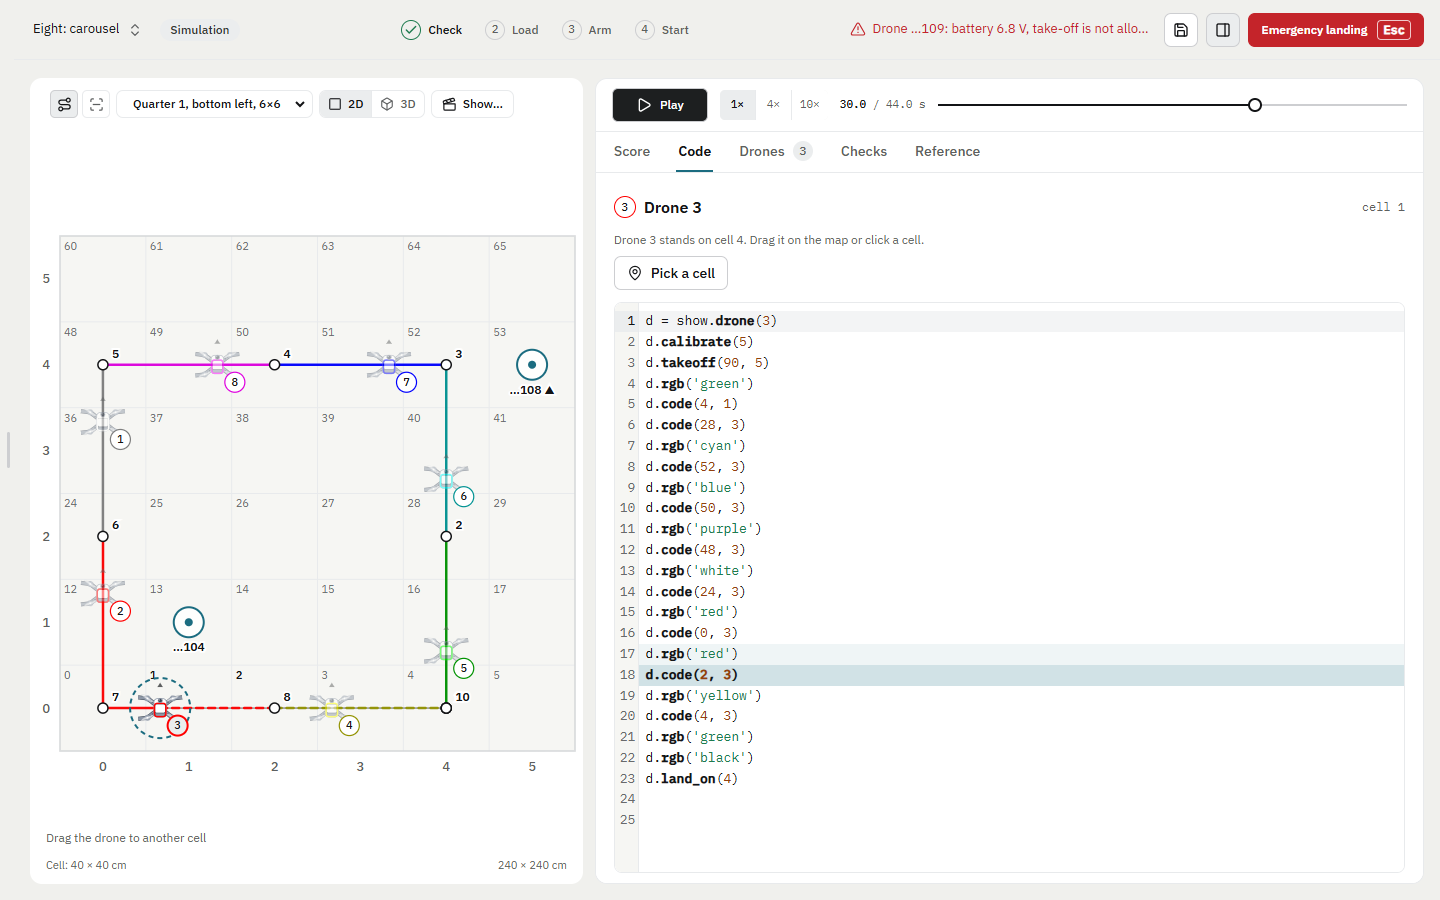
\includegraphics[width=\dimexpr\textwidth-2\fboxsep-2\fboxrule\relax]{figures/ide_simulation.png}}
\caption{Litebee IDE: симуляция шоу для нескольких дронов.}\label{fig:ide}
\end{figure}
